% CHAPTER 3 — PRODUCT DESIGN

\chapter{Product Design}

\section{Introduction}
This chapter presents the complete design of the BodyQ system at two
levels of abstraction. The high-level design section describes the
overall system architecture and the decomposition of the platform into
its major components. The detailed design section presents the key
interaction flows as sequence diagrams, the process models as activity
diagrams, and the data model as a class/entity description. The chapter
concludes with an overview of the user interface design.

\section{High-Level Design}

\subsection{Architecture Overview}
BodyQ is structured as a four-tier distributed system consisting of a
mobile client, a backend-as-a-service layer, a serverless AI engine
layer, and a web administration interface.

\begin{figure}[H]
	\centering
	\begin{tikzpicture}[
		node distance=1.5cm,
		box/.style={rectangle, draw=black, thick, fill=white, minimum width=3cm, minimum height=1cm, align=center, rounded corners},
		tier/.style={rectangle, draw=gray!50, dashed, fill=gray!5, minimum width=14.5cm, minimum height=2.2cm, anchor=west},
		label/.style={font=\bfseries\sffamily, color=gray!80}
		]
		
		% --- TIER 1: Presentation Layer ---
		\node[tier] (t1) at (0,0) {};
		\node[label, right=0.2cm of t1.north west, anchor=north west] {Tier 1: Presentation Layer};
		\node[box, fill=blue!10] (mobile) at (3.5,-1.1) {Mobile Client\\(Expo / React Native)};
		\node[box, fill=blue!10] (admin1) at (10.5,-1.1) {Web Dashboard\\(Next.js)};
		
		% --- TIER 2: Backend-as-a-Service ---
		\node[tier] (t2) at (0,-3) {};
		\node[label, right=0.2cm of t2.north west, anchor=north west] {Tier 2: Backend-as-a-Service (Supabase)};
		\node[box, fill=green!10, minimum width=2.5cm] (auth) at (2,-4.1) {Auth};
		\node[box, fill=green!10, minimum width=2.5cm] (api) at (5.5,-4.1) {PostgREST API};
		\node[box, fill=green!10, minimum width=2.5cm] (storage) at (9,-4.1) {Storage};
		\node[box, fill=green!10, minimum width=2.5cm] (edge) at (12.5,-4.1) {Edge Functions};
		
		% --- TIER 3: External Services ---
		\node[tier] (t3) at (0,-6) {};
		\node[label, right=0.2cm of t3.north west, anchor=north west] {Tier 3: External APIs \& CDNs};
		\node[box, fill=orange!10, minimum width=2.5cm] (groq) at (2,-7.1) {Groq\\(Llama-3.3)};
		\node[box, fill=orange!10, minimum width=2.5cm] (gemini) at (5.5,-7.1) {Gemini\\Vision};
		\node[box, fill=orange!10, minimum width=2.5cm] (off) at (9,-7.1) {Open Food\\Facts};
		\node[box, fill=orange!10, minimum width=2.5cm] (mp) at (12.5,-7.1) {MediaPipe\\CDN};
		
		% --- TIER 4: Administration ---
		\node[tier] (t4) at (0,-9) {};
		\node[label, right=0.2cm of t4.north west, anchor=north west] {Tier 4: Administration Infrastructure};
		\node[box, fill=purple!10, minimum width=6cm] (admin2) at (7.25,-10.1) {Admin Dashboard (React 18.0, Next.js 14)};
		
		% --- Connections ---
		\draw[thick, <->] (mobile) -- (api);
		\draw[thick, <->] (admin1) -- (api);
		\draw[thick, ->] (edge) -- (groq);
		\draw[thick, ->] (edge) -- (gemini);
		\draw[thick, ->] (mobile) -- (mp);
		\draw[thick, <->] (admin2) -- (api);
		
	\end{tikzpicture}
	\caption{BodyQ System Architecture: Four-Tier Layered Design}
	\label{fig:architecture}
\end{figure}

\textbf{Tier~1 --- Mobile Client (React Native / Expo SDK~54).}
The mobile application is built with React Native and Expo SDK~54 and
targets iOS~16+ and Android~11+. It is organized using the Expo Router
file-based navigation system. Application state is managed with Zustand
for global stores (authentication, user profile, active workout session)
and TanStack Query for server state and cache management. Forms are
handled with React Hook Form and validated using Zod schema definitions.

\textbf{Tier~2 --- Backend-as-a-Service (Supabase).}
Supabase provides the entire backend infrastructure: a managed
PostgreSQL~15 database, an authentication service (email/password and
Google OAuth~2.0), object storage for meal photos and profile images,
and Edge Functions running on the Deno runtime. Row Level Security
policies are applied to every table in the schema to enforce user data
isolation at the database level.

\textbf{Tier~3 --- AI Engine Layer.}
The AI engine is implemented as five Supabase Edge Functions:

\texttt{ai-assistant} (RAG conversational coaching)

\texttt{daily-tip} (daily AI insights)

\texttt{analyze-food} (meal photo recognition)

\texttt{generate-workout-plan} (personalized training programs)

\texttt{recommendation-engine} (rule-based recommendations).

These functions invoke the Claude API (Anthropic), the Groq inference platform(\texttt{llama-3.1-8b-instant}) or (\texttt{llama-3.3-70b-instant}), or the Google Gemini Vision API
depending on the task requirements and latency constraints.

\textbf{Tier~4 --- Administration Dashboard (React 18.0, Next.js~14).}
A web-based administration dashboard built with React 18.0, Next.js~14 (App Router) and Tailwind CSS provides operational management. 
All Supabase calls from the dashboard use the service role key exclusively via server-side Route Handlers.

% \subsection{Component Diagrams}
% TODO: UML Component diagram

\section{Detailed Design}

\subsection{Sequence Diagrams}
\textbf{SD-01: User Registration and AI-Personalized Onboarding.}

\begin{enumerate}
	\item User submits the registration form; mobile client calls
	\texttt{supabase.auth.signUp()}.
	\item Supabase Auth creates the user record and returns a session JWT.
	\item Mobile client navigates to onboarding; user completes all
	5~steps; collected data is buffered in a Zustand
	\texttt{onboardingStore}.
	\item On step~5 completion, the mobile client calls the
	\texttt{generate-workout-plan} Edge Function with the user profile
	JSON.
	\item The Edge Function invokes the Claude API and receives a
	personalized 4-week workout plan as structured JSON.
	\item The Edge Function computes BMR and TDEE; inserts records into
	\texttt{profiles} and \texttt{calorie\_targets}.
	\item The mobile client stores the plan and navigates to the Home tab.
\end{enumerate}

\textbf{SD-02: RAG Coaching Pipeline (Yara AI Assistant).}

\begin{enumerate}[noitemsep]
	\item User types a question in the AI assistant chat screen.
	\item Mobile client calls
	\texttt{supabase.functions.invoke('ai-assistant')} with
	\texttt{\{userId, query\}}.
	\item \textbf{Retrieve:} Edge Function executes four SQL queries---7-day
	\texttt{daily\_activity} window, 7-day \texttt{food\_logs}
	aggregated by day, active \texttt{calorie\_targets}, and last~5
	\texttt{workout\_sessions}.
	\item \textbf{Augment:} Retrieved records are formatted into a
	structured plain-text context block; out-of-range values (e.g.,
	sleep $<6$\,h, hydration $<1500$\,mL) are flagged with warning
	markers; four behavioral rules are appended.
	\item \textbf{Generate:} Augmented prompt is sent to the Groq API
	(\texttt{Llama3.3 70b}).
	\item Edge Function inserts the response into \texttt{ai\_insights}
	(\texttt{type='chat'}) and returns it to the mobile client.
\end{enumerate}

\textbf{SD-03: Posture Detection During Workout.}

\begin{enumerate}[noitemsep]
	\item User taps ``PostureAI'' during an active workout session.
	\item Mobile client renders \texttt{PostureScreen} with an Expo
	WebView component.
	\item WebView HTML loads MediaPipe Pose JS from CDN, initializes the
	model, and starts the device camera via \texttt{getUserMedia}.
	\item At each video frame, MediaPipe detects 33~landmarks; the array
	is serialized to JSON and posted to React Native via
	\texttt{window.ReactNativeWebView.postMessage()}.
	\item \texttt{PostureEngine.analyzeSquat(landmarks)} is called; joint
	angles are computed using the vector dot-product formula and
	evaluated against reference ranges; rep direction changes are
	tracked.
	\item Score, feedback strings, and rep count are rendered on the
	overlay UI in real time.
\end{enumerate}

\subsection{Activity Diagrams}
% TODO: Workout session flow, onboarding 

\textbf{AD-01: Workout Session Flow.}

The activity diagram in Figure~\ref{fig:ad-workout} models the
lifecycle of a single workout session from the moment the user opens
the Training tab to the persistence of the completed session.

The flow begins when the user opens the Training tab and the
\texttt{useWorkout} hook loads the exercise library from Supabase.
The user may search or browse the library and then taps ``Start
Workout'', which starts the session timer and initialises an empty
exercise list in local state.

Inside the session the user enters a loop: they select an exercise
from the library, record one or more sets with reps and weight for
each, and then decide whether to add another exercise. This loop
repeats until the user taps ``Finish Workout''. At that point the
system stops the timer, calculates total duration and estimated
calories burned, and calls \texttt{workoutService.saveSession()} to
persist a \texttt{workout\_sessions} row with the exercises encoded
as a JSONB array. The user is then navigated to the
\texttt{WorkoutSummary} screen, which displays duration, exercises
completed, and estimated calories. Tapping ``Done'' returns the user
to the Training tab.

\begin{figure}[H]
	\centering
	\begin{tikzpicture}[scale=0.8, transform shape,
		node distance=1.5cm,
		auto,
		startstop/.style={draw, circle, fill=black, minimum size=10pt, inner sep=0pt},
		endstop/.style={draw, double, circle, fill=black, minimum size=10pt, inner sep=2pt},
		activity/.style={rectangle, draw, thick, rounded corners, fill=white, minimum width=3.5cm, minimum height=1cm, align=center, font=\small},
		decision/.style={diamond, draw, thick, fill=white, aspect=1.5, minimum width=2cm, font=\scriptsize},
		line/.style={draw, thick, -{Stealth[scale=1.2]}},
		swimlane/.style={draw, gray!30, line width=0.5pt}]
		% --- SWIMLANES ---
		\draw[swimlane] (-1, 1) -- (-1, -16); 
		\draw[swimlane] (5, 1) -- (5, -16);   
		\draw[swimlane] (11, 1) -- (11, -16); 
		\node[font=\Large\bfseries] at (2, 0.5) {User};
		\node[font=\Large\bfseries] at (8, 0.5) {System};
		% --- NODES ---
		\node[startstop] (start) at (2, 0) {};
		\node[activity, below=0.6cm of start] (start_sess) {Select "Start Workout"};
		\node[activity] (init) at (8, -1.6) {Initialize Session \&\\Record Start Time};
		\node[activity] (select) at (2, -3.5) {Search \& Select\\Exercise from Library};
		\node[activity, below=1.2cm of select] (log) {Log Sets\\(Reps, Weight, RPE)};
		\node[decision, below=1.2cm of log] (another) {Add another\\exercise?};
		\node[activity, below=1.5cm of another] (finish) {Select "Finish Workout"};
		\node[activity] (calc) at (8, -10.5) {Calculate Duration,\\Volume \& Calories};
		\node[activity, below=1.2cm of calc] (save) {Persist Session to\\Supabase Database};
		\node[activity] (summary) at (2, -13.3) {View Workout\\Summary Screen};
		\node[endstop, below=0.8cm of summary] (end) {};
		% --- CONNECTIONS ---
		\draw[line] (start) -- (start_sess);
		\draw[line] (start_sess) -- (init);
		\draw[line] (init.south) |- (select.east);
		\draw[line] (select) -- (log);
		\draw[line] (log) -- (another);
		\draw[line] (another.west) -- ++(-1,0) node[above, pos=0.5] {Yes} |- (select.west);
		\draw[line] (another) -- node[right] {No} (finish);
		\draw[line] (finish) -- (calc);
		\draw[line] (calc) -- (save);
		\draw[line] (save) -- (summary);
		\draw[line] (summary) -- (end);
	\end{tikzpicture}
	\caption{AD-01: Workout session activity diagram showing exercise logging loop.}
	\label{fig:ad-workout}
\end{figure}

\textbf{AD-02: Onboarding Flow.}

Figure~\ref{fig:ad-onboarding} describes the onboarding process that
executes once after a user's first successful registration.

After registration, Supabase Auth fires a database trigger that
inserts a skeleton row into \texttt{profiles}. The mobile client
detects the empty profile and redirects to the first onboarding
screen. The user progresses through five data-collection steps:
personal data (age, sex), body measurements (height, current weight),
fitness goal selection (weight loss, muscle gain, or maintenance),
activity level, and training experience level. Each step validates
its inputs locally; the user cannot advance until all required fields
are complete.

On completion of step~5 the system forks into two concurrent
branches. The first branch calls \texttt{macroCalc.calculateTDEE()}
with the collected profile data, computes the Basal Metabolic Rate
using the Mifflin-St\,Jeor equation, and writes the resulting calorie
and macro targets to \texttt{profiles} and \texttt{calorie\_targets}.
The second branch invokes the \texttt{generate-workout-plan} Edge
Function, which calls the Claude API and stores the returned
four-week training programme as a JSONB document in
\texttt{profiles.workout\_plan}. Both branches must complete before
the flow joins and navigates the user to the Home tab for the first
time.

If the user declines to enable cycle tracking during onboarding the
\texttt{cycle\_tracking\_enabled} flag is set to \texttt{false} and
the cycle-phase recommendation logic is bypassed throughout the
application.

\begin{figure}[H]
	\centering
	% Resizebox ensures it fits the page width perfectly
	\resizebox{\textwidth}{!}{
		\begin{tikzpicture}[
			node distance=1.8cm, % Increased distance to prevent overlap
			auto,
			% Styles
			startstop/.style={draw, circle, fill=black, minimum size=10pt, inner sep=0pt},
			endstop/.style={draw, double, circle, fill=black, minimum size=10pt, inner sep=2pt},
			activity/.style={rectangle, draw, thick, rounded corners, fill=white, minimum width=3.5cm, minimum height=1cm, align=center, font=\small},
			decision/.style={diamond, draw, thick, fill=white, aspect=1.5, minimum width=1.8cm, font=\scriptsize},
			sync/.style={rectangle, fill=black, minimum width=7cm, minimum height=3pt, inner sep=0pt},
			line/.style={draw, thick, -{Stealth[scale=1.2]}},
			swimlane/.style={draw, gray!30, line width=0.5pt}
			]
			
			% --- SWIMLANES ---
			% Vertical lines
			\draw[swimlane] (-1, 1) -- (-1, -18);
			\draw[swimlane] (5, 1) -- (5, -18);
			\draw[swimlane] (12, 1) -- (12, -18);
			
			% Headers
			\node[font=\Large\bfseries] at (2, 0.5) {User};
			\node[font=\Large\bfseries] at (8.5, 0.5) {System};
			
			% --- USER LANE NODES ---
			\node[startstop] (start) at (2, 0) {};
			
			\node[activity, below=0.8cm of start] (step1) {Step 1: Basic Info\\(Age, Sex, Height)};
			\node[decision, below=0.8cm of step1] (dec1) {Valid?};
			
			\node[activity, below=1.2cm of dec1] (step2to4) {Steps 2--4: Metrics\\(Weight, Goal, Activity)};
			\node[decision, below=0.8cm of step2to4] (dec2) {Valid?};
			
			\node[activity, below=1.2cm of dec2] (step5) {Step 5: Experience\\(Training Level)};
			\node[decision, below=0.8cm of step5] (dec3) {Valid?};
			
			% --- SYSTEM LANE NODES ---
			% Fork bar
			\node[sync] (fork) at (8.5, -9.5) {};
			
			% Branch A (Left side of System lane)
			\node[activity, below=1.5cm of fork, xshift=-2cm] (calc) {Calculate BMR/TDEE\\(Mifflin-St Jeor)};
			\node[activity, below=1.2cm of calc] (writeA) {Write to \texttt{profiles} \&\\\texttt{calorie\_targets}};
			
			% Branch B (Right side of System lane)
			\node[activity, below=1.5cm of fork, xshift=2cm] (edge) {Invoke Edge Function\\(Claude API)};
			\node[activity, below=1.2cm of edge] (writeB) {Write to\\\texttt{workout\_plan}};
			
			% Join bar
			\node[sync] (join) at (8.5, -15) {};
			
			% Final Navigation
			\node[activity, below=1cm of join] (home) {Navigate to Home Dashboard};
			\node[endstop, below=0.8cm of home] (end) {};
			
			% --- CONNECTIONS ---
			
			% Main Flow (User)
			\draw[line] (start) -- (step1);
			\draw[line] (step1) -- (dec1);
			\draw[line] (dec1) -- node[right] {Yes} (step2to4);
			\draw[line] (step2to4) -- (dec2);
			\draw[line] (dec2) -- node[right] {Yes} (step5);
			\draw[line] (step5) -- (dec3);
			
			% Validation Loops (No paths) - Routed to the left to avoid clutter
			\draw[line] (dec1.west) -- ++(-0.8,0) |- node[left, pos=0.2] {No} (step1.west);
			\draw[line] (dec2.west) -- ++(-0.8,0) |- node[left, pos=0.2] {No} (step2to4.west);
			\draw[line] (dec3.west) -- ++(-0.8,0) |- node[left, pos=0.2] {No} (step5.west);
			
			% Transition to System
			\draw[line] (dec3.east) -- node[above, pos=0.2] {Yes} (fork.west);
			
			% Parallel Processing
			\draw[line] (fork.south -| calc) -- (calc.north);
			\draw[line] (fork.south -| edge) -- (edge.north);
			\draw[line] (calc) -- (writeA);
			\draw[line] (edge) -- (writeB);
			
			% Join
			\draw[line] (writeA.south) -- (join.north -| writeA.south);
			\draw[line] (writeB.south) -- (join.north -| writeB.south);
			
			% Final
			\draw[line] (join) -- (home);
			\draw[line] (home) -- (end);
			
		\end{tikzpicture}
	}
	\caption{AD-02: User onboarding activity diagram with parallel system logic.}
	\label{fig:ad-onboarding}
\end{figure}

\subsection{Class Diagram}
% TODO: Based on DB schema

Figure~\ref{fig:class} presents the domain model as a UML class
diagram. Because BodyQ is implemented in JavaScript and TypeScript
rather than a classical object-oriented language, the diagram
represents logical data shapes and the modules that own them rather
than an inheritance hierarchy.

The central class is \textbf{UserProfile}, which extends Supabase's
built-in \texttt{auth.users} entity via a one-to-one foreign key on
\texttt{id}. It stores all biometric and preference attributes derived
during onboarding (age, sex, height, weight, goal, activity level,
experience level), the computed targets (calorie, protein,
carbohydrates, fat, and water), and the AI-generated workout plan
encoded as a JSONB document.

\textbf{FoodLog} records a single food item consumed by the user,
capturing food name, macro values, meal type, and timestamp. Many
\texttt{FoodLog} instances belong to one \texttt{UserProfile}.
\textbf{CalorieTarget} stores a date-stamped snapshot of the user's
macro targets, enabling the correlation engine to join targets to
activity records by date without referencing the mutable profile
row.

\textbf{WorkoutSession} records a completed training session. It
holds session metadata (start time, end time, duration) and
aggregates its exercises via a composition relationship with
\textbf{ExerciseEntry}, which in turn composes one or more
\textbf{SetRecord} value objects. The \texttt{exercises} column in
the database is a JSONB array that serialises this nested structure
as a single column.

\textbf{DailyActivity} is the central fact table for the correlation
engine. It stores one row per user per day, recording steps, water
intake, sleep hours, and the current menstrual cycle phase for
eligible users. \textbf{CycleLog} tracks individual phase
transitions for users who have enabled cycle tracking.

\textbf{AIInsight} persists every coaching response and daily tip
generated by the Yara assistant or the \texttt{daily-tip} Edge
Function, allowing historical insights to be replayed in the chat
interface.

The \textbf{PostureEngine} module (shown as a utility class) is
stateless; it accepts a landmark array and an exercise identifier and
returns a \texttt{PostureResult} value object. The
\textbf{MacroCalc} utility is a pure-function module with no database
dependencies; its three public methods implement the
Mifflin-St\,Jeor BMR formula, the TDEE multiplier, and the
goal-adjusted macro split.

\begin{figure}[H]
	\centering
	\resizebox{\textwidth}{!}{
		\begin{tikzpicture}[
			node distance=1.5cm,
			>=Stealth,
			% Class Box Style
			class/.style={
				draw, rectangle split, rectangle split parts=2, 
				fill=white, thick, anchor=center, text width=4.5cm, font=\footnotesize
			},
			% Utility Style (3 parts for methods)
			utility/.style={
				draw, rectangle split, rectangle split parts=3, 
				fill=gray!5, thick, anchor=center, text width=5.5cm, font=\footnotesize
			},
			% Association Styles
			oneToMany/.style={draw, thick, {Straight Barb[reversed]}-},
			composition/.style={draw, thick, {Diamond[fill=black]}-},
			dependency/.style={draw, thick, dashed, ->}
			]
			
			% --- CENTRAL CLASS ---
			\node[class, text width=5cm] (UserProfile) {
				\textbf{UserProfile}
				\nodepart{second}
				id : UUID \\ fullName : String \\ age : Int \\ sex : String \\ weightKg : Float \\ heightCm : Float \\ goal : String \\ activityLevel : String \\ experienceLevel : String \\ calorieTarget : Int \\ proteinTarget : Int \\ carbsTarget : Int \\ fatTarget : Int \\ waterTargetMl : Int \\ cycleTrackingEnabled : Bool \\ workoutPlan : JSON
			};
			
			% --- LEFT COLUMN: Nutrition & Tracking ---
			\node[class, left=3cm of UserProfile, yshift=4cm] (FoodLog) {
				\textbf{FoodLog}
				\nodepart{second}
				id : UUID \\ userId : UUID \\ foodName : String \\ calories : Int \\ protein : Int \\ carbs : Int \\ fat : Int \\ mealType : String \\ loggedAt : DateTime
			};
			
			\node[class, left=3cm of UserProfile, yshift=0cm] (CalorieTarget) {
				\textbf{CalorieTarget}
				\nodepart{second}
				id : UUID \\ userId : UUID \\ date : Date \\ calorieTarget : Int \\ proteinTarget : Int \\ carbsTarget : Int \\ fatTarget : Int
			};
			
			\node[class, left=3cm of UserProfile, yshift=-4cm] (DailyActivity) {
				\textbf{DailyActivity}
				\nodepart{second}
				userId : UUID \\ date : Date \\ steps : Int \\ waterMl : Int \\ sleepHours : Float \\ cyclePhase : String
			};
			
			\node[class, left=5.5cm of DailyActivity, yshift=0cm] (CycleLog) {
				\textbf{CycleLog}
				\nodepart{second}
				id : UUID \\ userId : UUID \\ phase : String \\ loggedDate : Date
			};
			
			% --- RIGHT COLUMN: Workouts ---
			\node[class, right=3cm of UserProfile, yshift=2cm] (WorkoutSession) {
				\textbf{WorkoutSession}
				\nodepart{second}
				id : UUID \\ userId : UUID \\ name : String \\ startedAt : DateTime \\ endedAt : DateTime \\ durationMinutes : Int
			};
			
			\node[class, below=1.5cm of WorkoutSession] (ExerciseEntry) {
				\textbf{ExerciseEntry}
				\nodepart{second}
				exerciseId : UUID \\ name : String \\ muscleGroup : String
			};
			
			\node[class, below=1.5cm of ExerciseEntry] (SetRecord) {
				\textbf{SetRecord}
				\nodepart{second}
				reps : Int \\ weightKg : Float
			};
			
			% --- BOTTOM: AI & Insights ---
			\node[class, below=3cm of UserProfile] (AIInsight) {
				\textbf{AIInsight}
				\nodepart{second}
				id : UUID \\ userId : UUID \\ content : Text \\ type : [tip|chat] \\ tone : String \\ createdAt : DateTime
			};
			
			% --- UTILITIES (Top and Far Right) ---
			\node[utility, above=2cm of UserProfile] (MacroCalc) {
				\textbf{\guillemotleft utility\guillemotright \\ MacroCalc}
				\nodepart{second}
				\nodepart{third}
				+ calculateBMR(profile) \\ + calculateTDEE(bmr, activity) \\ + calculateMacros(tdee, goal)
			};
			
			\node[utility, right=1.5cm of WorkoutSession, xshift=1cm] (PostureEngine) {
				\textbf{\guillemotleft utility\guillemotright \\ PostureEngine}
				\nodepart{second}
				\nodepart{third}
				+ analyseFrame(landmarks, ex) \\ - computeAngle(a, b, c) \\ - evaluateForm(angles, ex) \\ - detectRepCycle(angle, hist)
			};
			
			% --- ASSOCIATIONS ---
			
			% UserProfile 1 -- *
			\draw[oneToMany] (UserProfile.west) -- ++(-1,0) |- (FoodLog.east) node[pos=0.9, above] {*};
			\draw[oneToMany] (UserProfile.west) -- (CalorieTarget.east) node[pos=0.9, above] {*};
			\draw[oneToMany] (UserProfile.west) -- ++(-1,0) |- (DailyActivity.east) node[pos=0.9, above] {*};
			\draw[oneToMany] (DailyActivity.west) -- (CycleLog.east) node[pos=0.9, above] {*};
			\draw[oneToMany] (UserProfile.east) -- (WorkoutSession.west) node[pos=0.9, above] {*};
			\draw[oneToMany] (UserProfile.south) -- (AIInsight.north) node[pos=0.9, right] {*};
			
			% Composition (Workout Hierarchy)
			\draw[composition] (WorkoutSession.south) -- (ExerciseEntry.north) node[pos=0.1, right] {1} node[pos=0.9, right] {*};
			\draw[composition] (ExerciseEntry.south) -- (SetRecord.north) node[pos=0.1, right] {1} node[pos=0.9, right] {*};
			
			% Dependencies
			\draw[dependency] (MacroCalc.south) -- (UserProfile.north) node[midway, right] {computes targets};
			\draw[dependency] (PostureEngine.west) -- (WorkoutSession.east) node[midway, above] {contributes data};
			
			% Multiplicity 1s
			\node[above right=0.1cm of UserProfile.west, font=\scriptsize] {1};
			\node[above left=0.1cm of UserProfile.east, font=\scriptsize] {1};
			\node[below right=0.1cm of UserProfile.south, font=\scriptsize] {1};
			
		\end{tikzpicture}
	}
	\caption{BodyQ domain model class diagram.}
	\label{fig:class}
\end{figure}


\section{UI Design}
% TODO: Wireframes / mockups

\subsection{Design Principles}

The BodyQ interface is built on four guiding principles that address
the usability gaps identified in the competitive analysis in
Chapter~1.

\textbf{Dark-first aesthetics.} The application enforces a dark colour
scheme globally (\texttt{userInterfaceStyle: "dark"} in
\texttt{app.json}). The primary background colour is
\texttt{\#0F0B1E} (deep indigo) with purple and teal accent colours.
This reduces eye strain during low-light training sessions and aligns
the product visually with premium fitness applications.

\textbf{Progressive disclosure.} Complex outputs such as correlation
insights, cycle-phase adjustments, and AI coaching reasoning are
surfaced only when the user navigates to them. The Home tab presents
only the most critical daily metrics (calories, macros, water, and
steps) as ring-chart and stat-card primitives. Advanced analytics
are accessible via the Insights sub-screen.

\textbf{Minimal input friction.} Every food-logging path---barcode
scan, AI photo recognition, and text search---is designed to minimise
the number of taps required before a meal is confirmed. The
\texttt{FoodResultSheet} bottom sheet pre-populates all fields from
the recognition pipeline so the user only needs to adjust portion
size if required.

\textbf{Contextual feedback.} The PostureAI overlay and the Yara
coaching interface both tie their output directly to what the user is
doing at that moment. Posture scores update in real time during a
set; AI coaching responses are grounded in the user's own recent data
so that advice is never generic.

\subsection{Navigation Structure}

The application uses a five-tab bottom navigation bar, implemented
with Expo Router's tab layout. Table~\ref{tab:navigation} summarises
each tab, its primary screen component, and its key child screens.

\begin{table}[H]
	\centering
	\caption{Application navigation structure}
	\label{tab:navigation}
	\begin{tabularx}{\textwidth}{llX}
		\toprule
		\textbf{Tab} & \textbf{Root Screen} & \textbf{Child Screens / Overlays} \\
		\midrule
		Home      & \texttt{Home.js}       & Daily AI tip card, macro detail modal \\
		Nutrition & \texttt{Nutrition.js}  & \texttt{MealLogger.js}, \texttt{FoodScannerScreen.js},
		\texttt{FoodResultSheet} (bottom sheet) \\
		Training  & \texttt{Training.js}   & \texttt{WorkoutActive.js},
		\texttt{WorkoutSummary.js},
		\texttt{PostureAI.js} (overlay) \\
		Insights  & \texttt{Insights.js}   & Correlation cards, weekly charts \\
		Profile   & \texttt{Profile.js}    & \texttt{SleepLog.js},
		\texttt{YaraAssistant.js} (chat),
		cycle log, streak history \\
		\bottomrule
	\end{tabularx}
\end{table}

\subsection{Key Screens}

\begin{figure}[H]
	\centering
	% --- ROW 1 ---
	\begin{subfigure}[b]{0.31\textwidth}
		\centering
		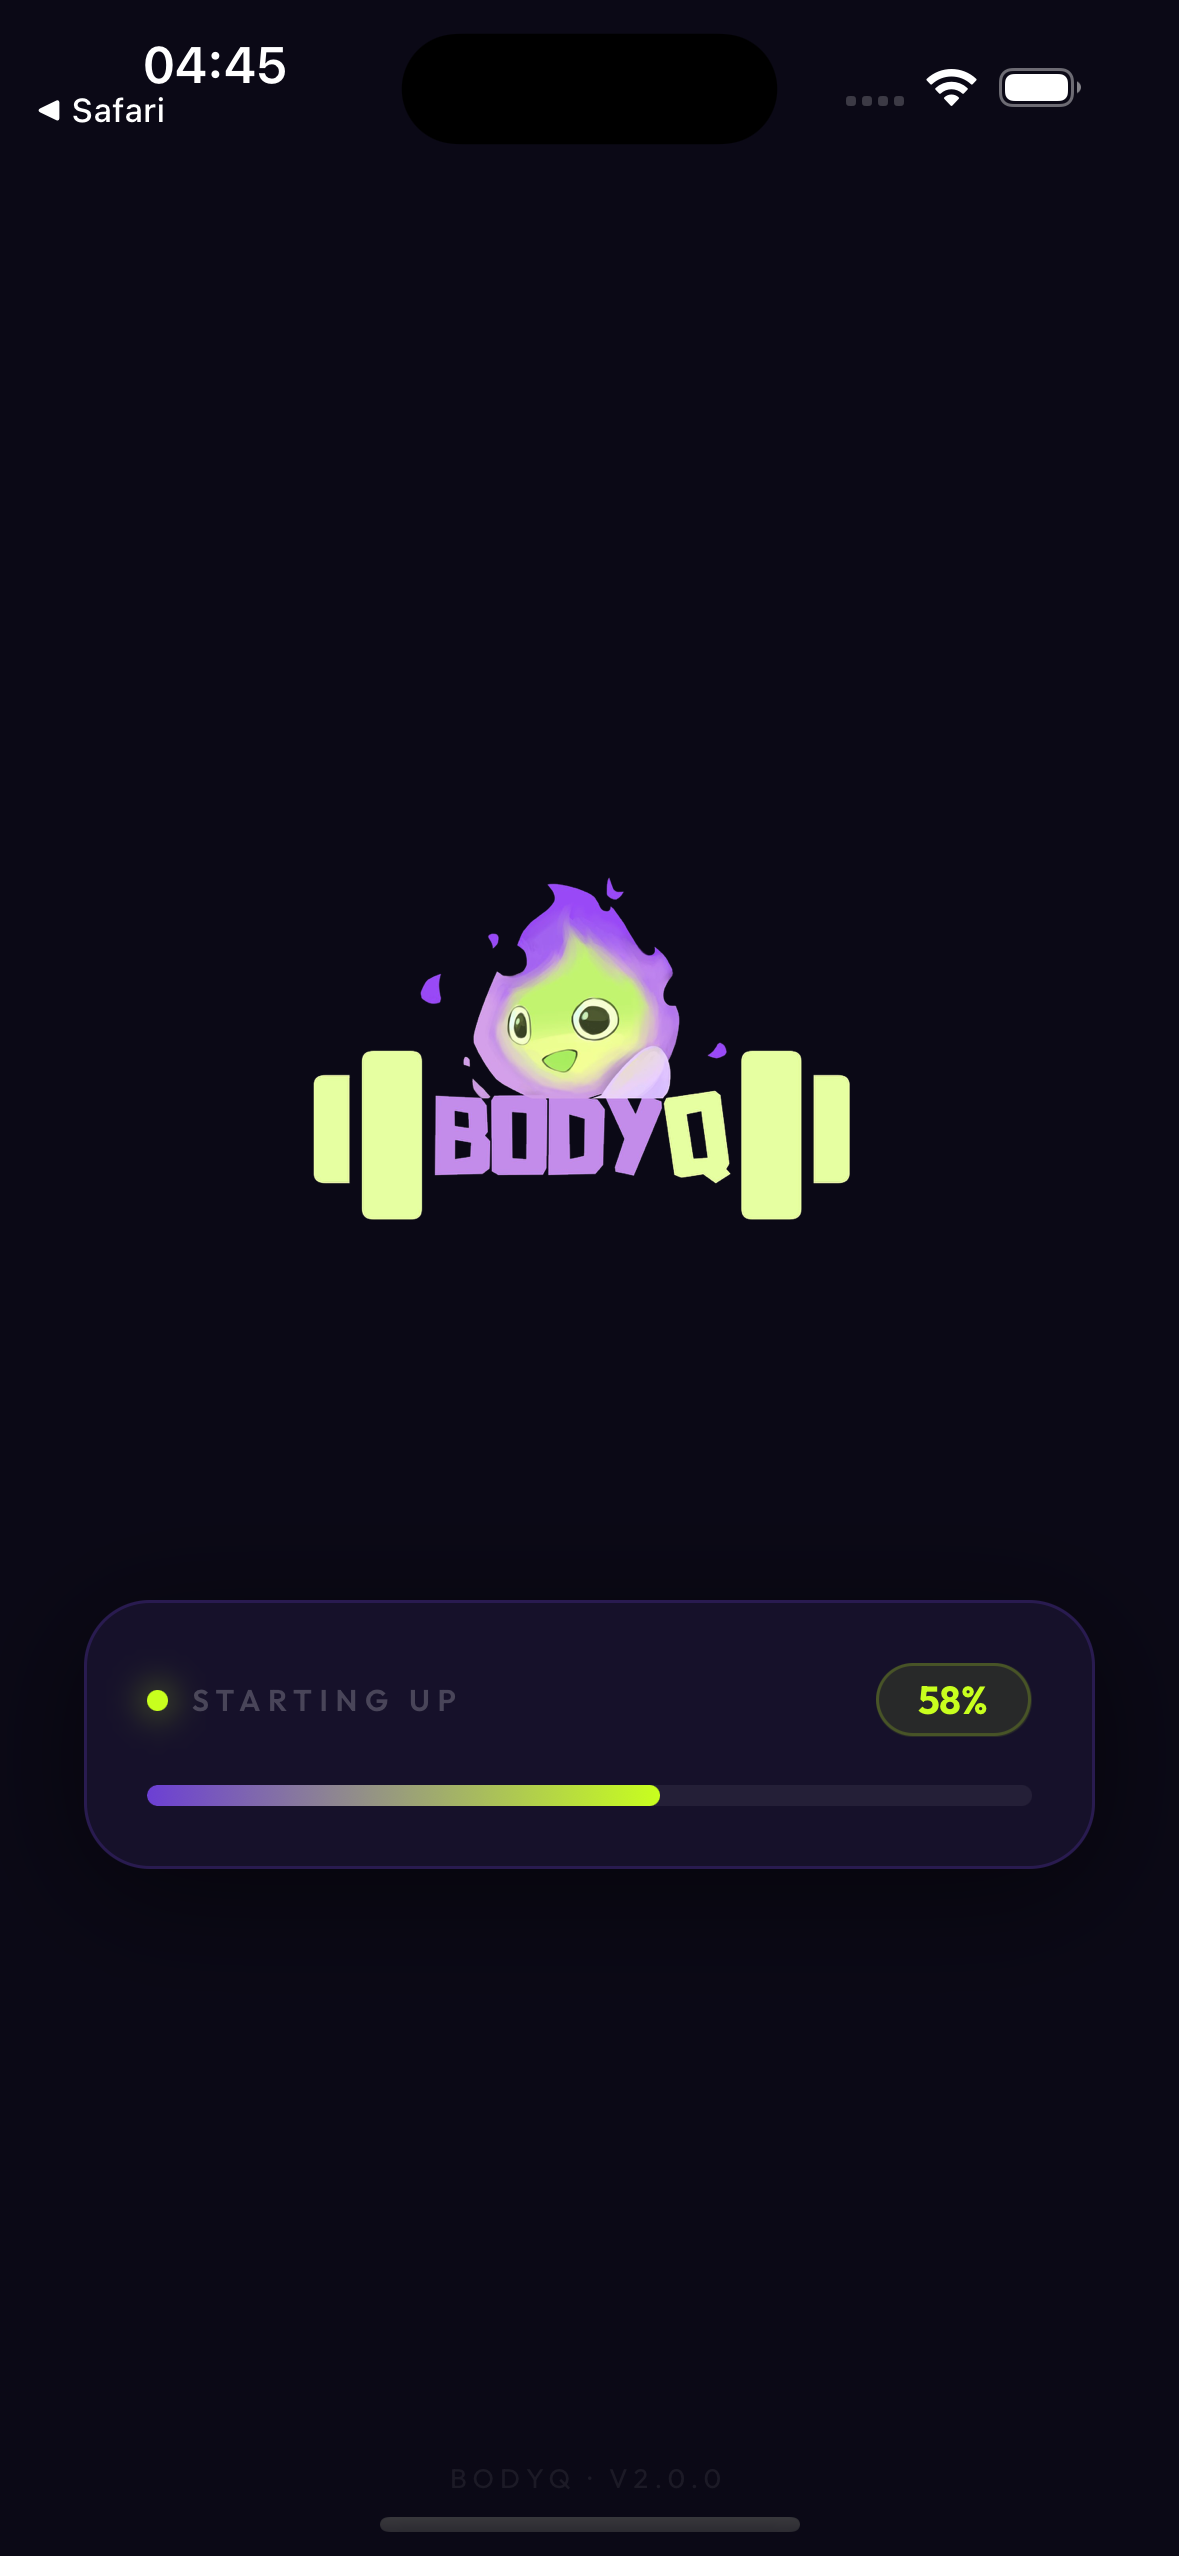
\includegraphics[width=\textwidth]{images/launch-screen}
		\caption{Launch Screen}
		\label{fig:ui-launch}
	\end{subfigure}
	\hfill
	\begin{subfigure}[b]{0.31\textwidth}
		\centering
		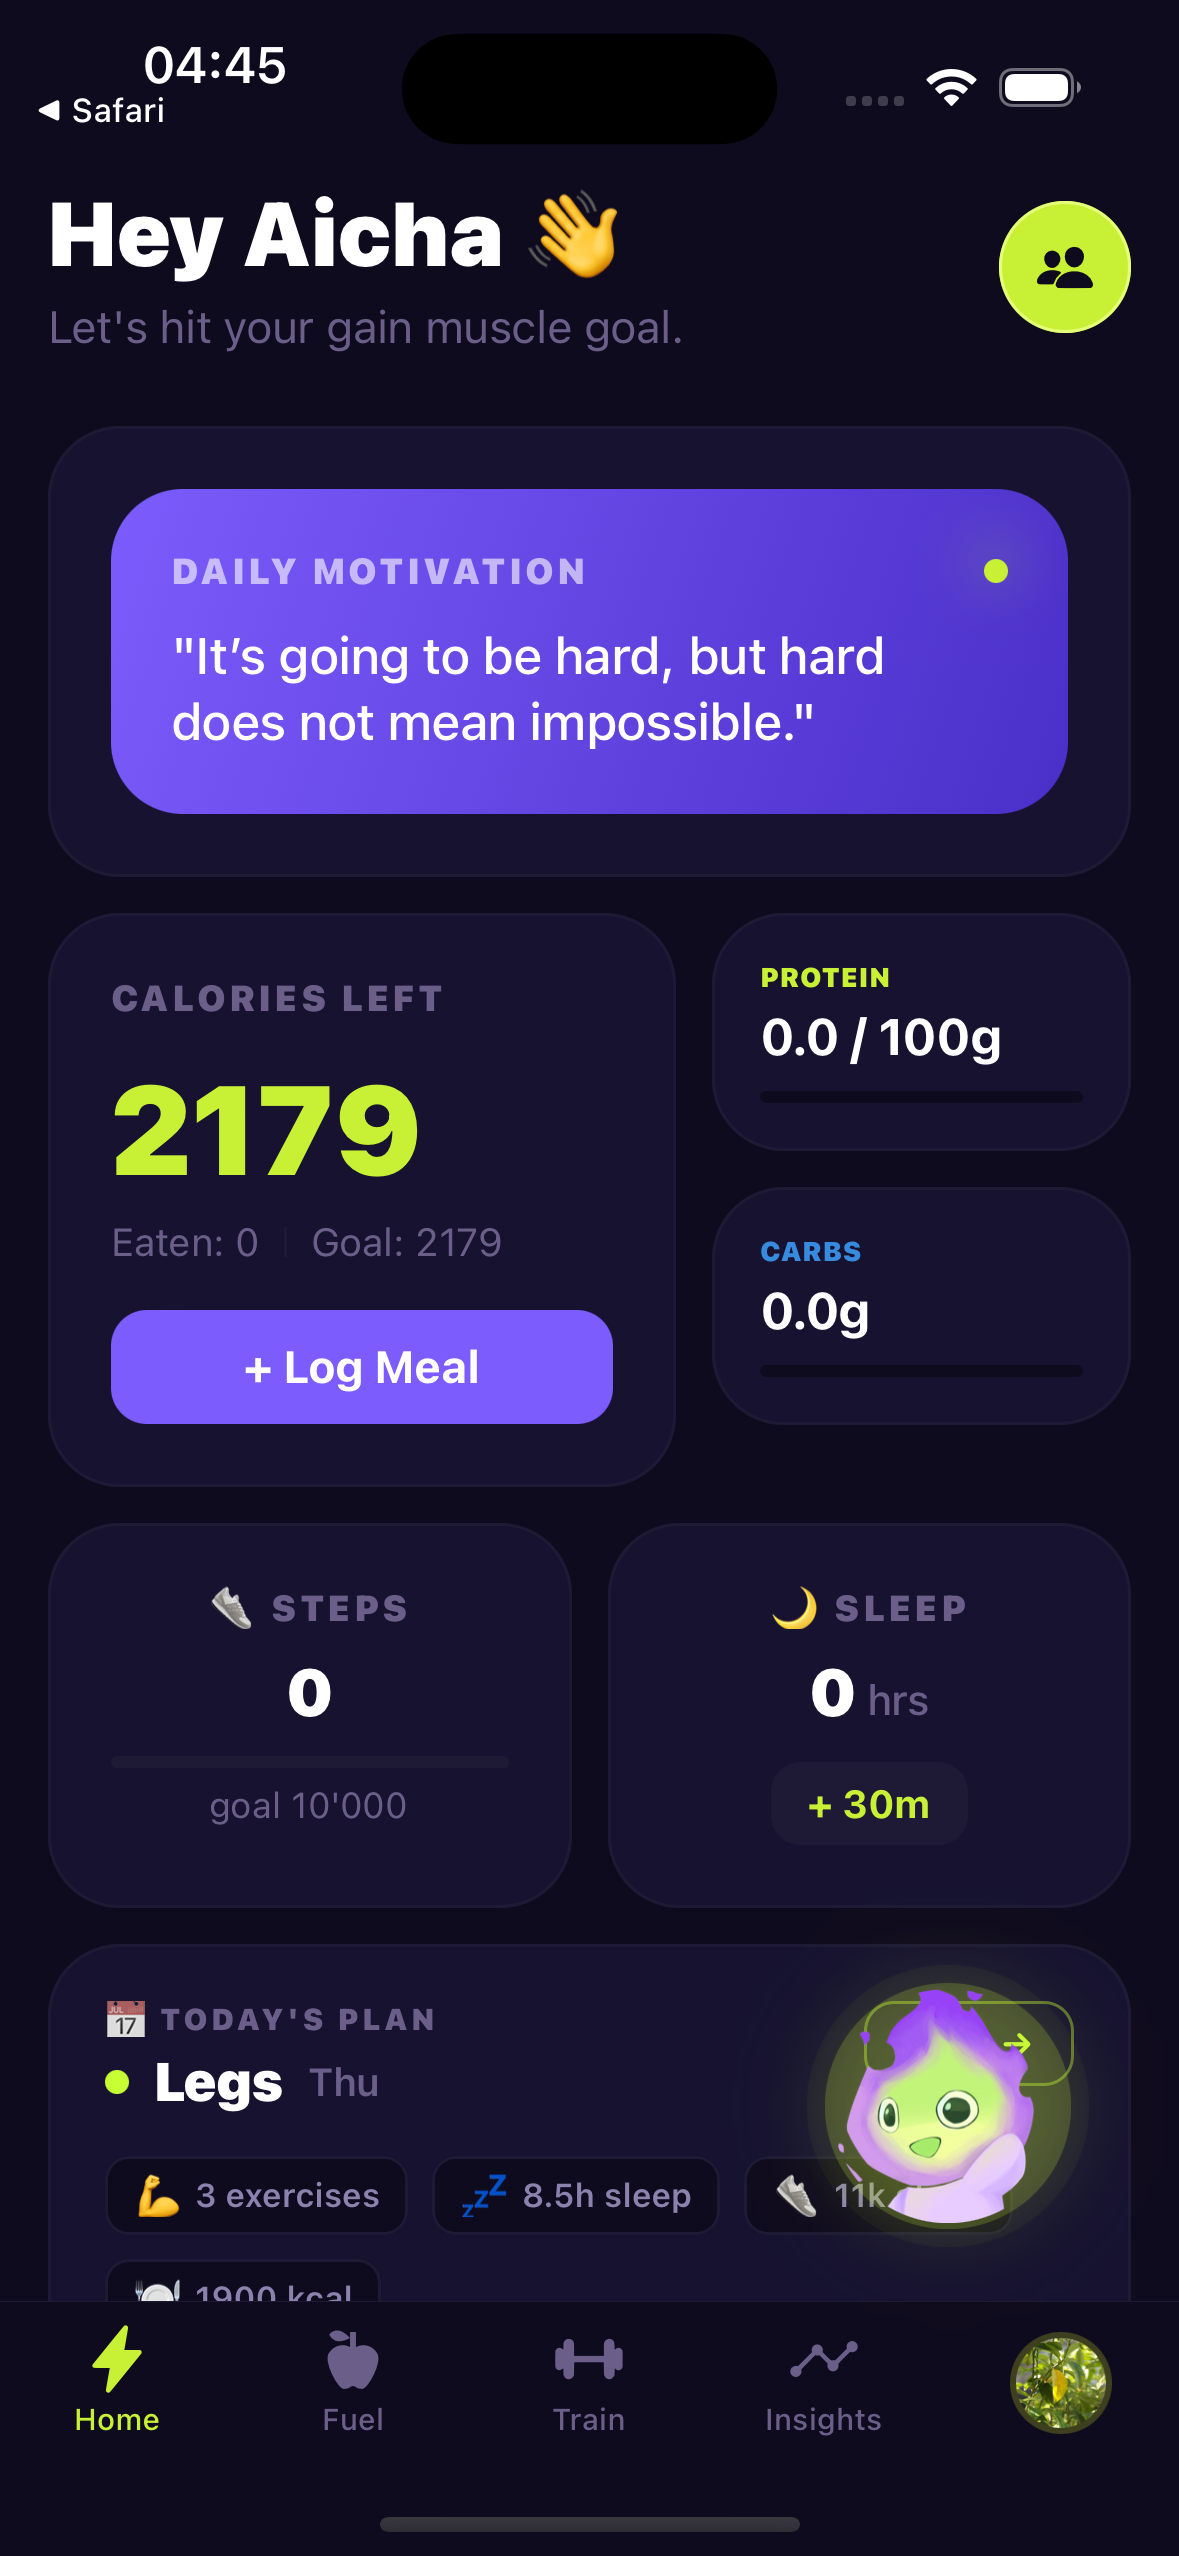
\includegraphics[width=\textwidth]{images/home-screen}
		\caption{Home Dashboard}
		\label{fig:ui-home}
	\end{subfigure}
	\hfill
	\begin{subfigure}[b]{0.31\textwidth}
		\centering
		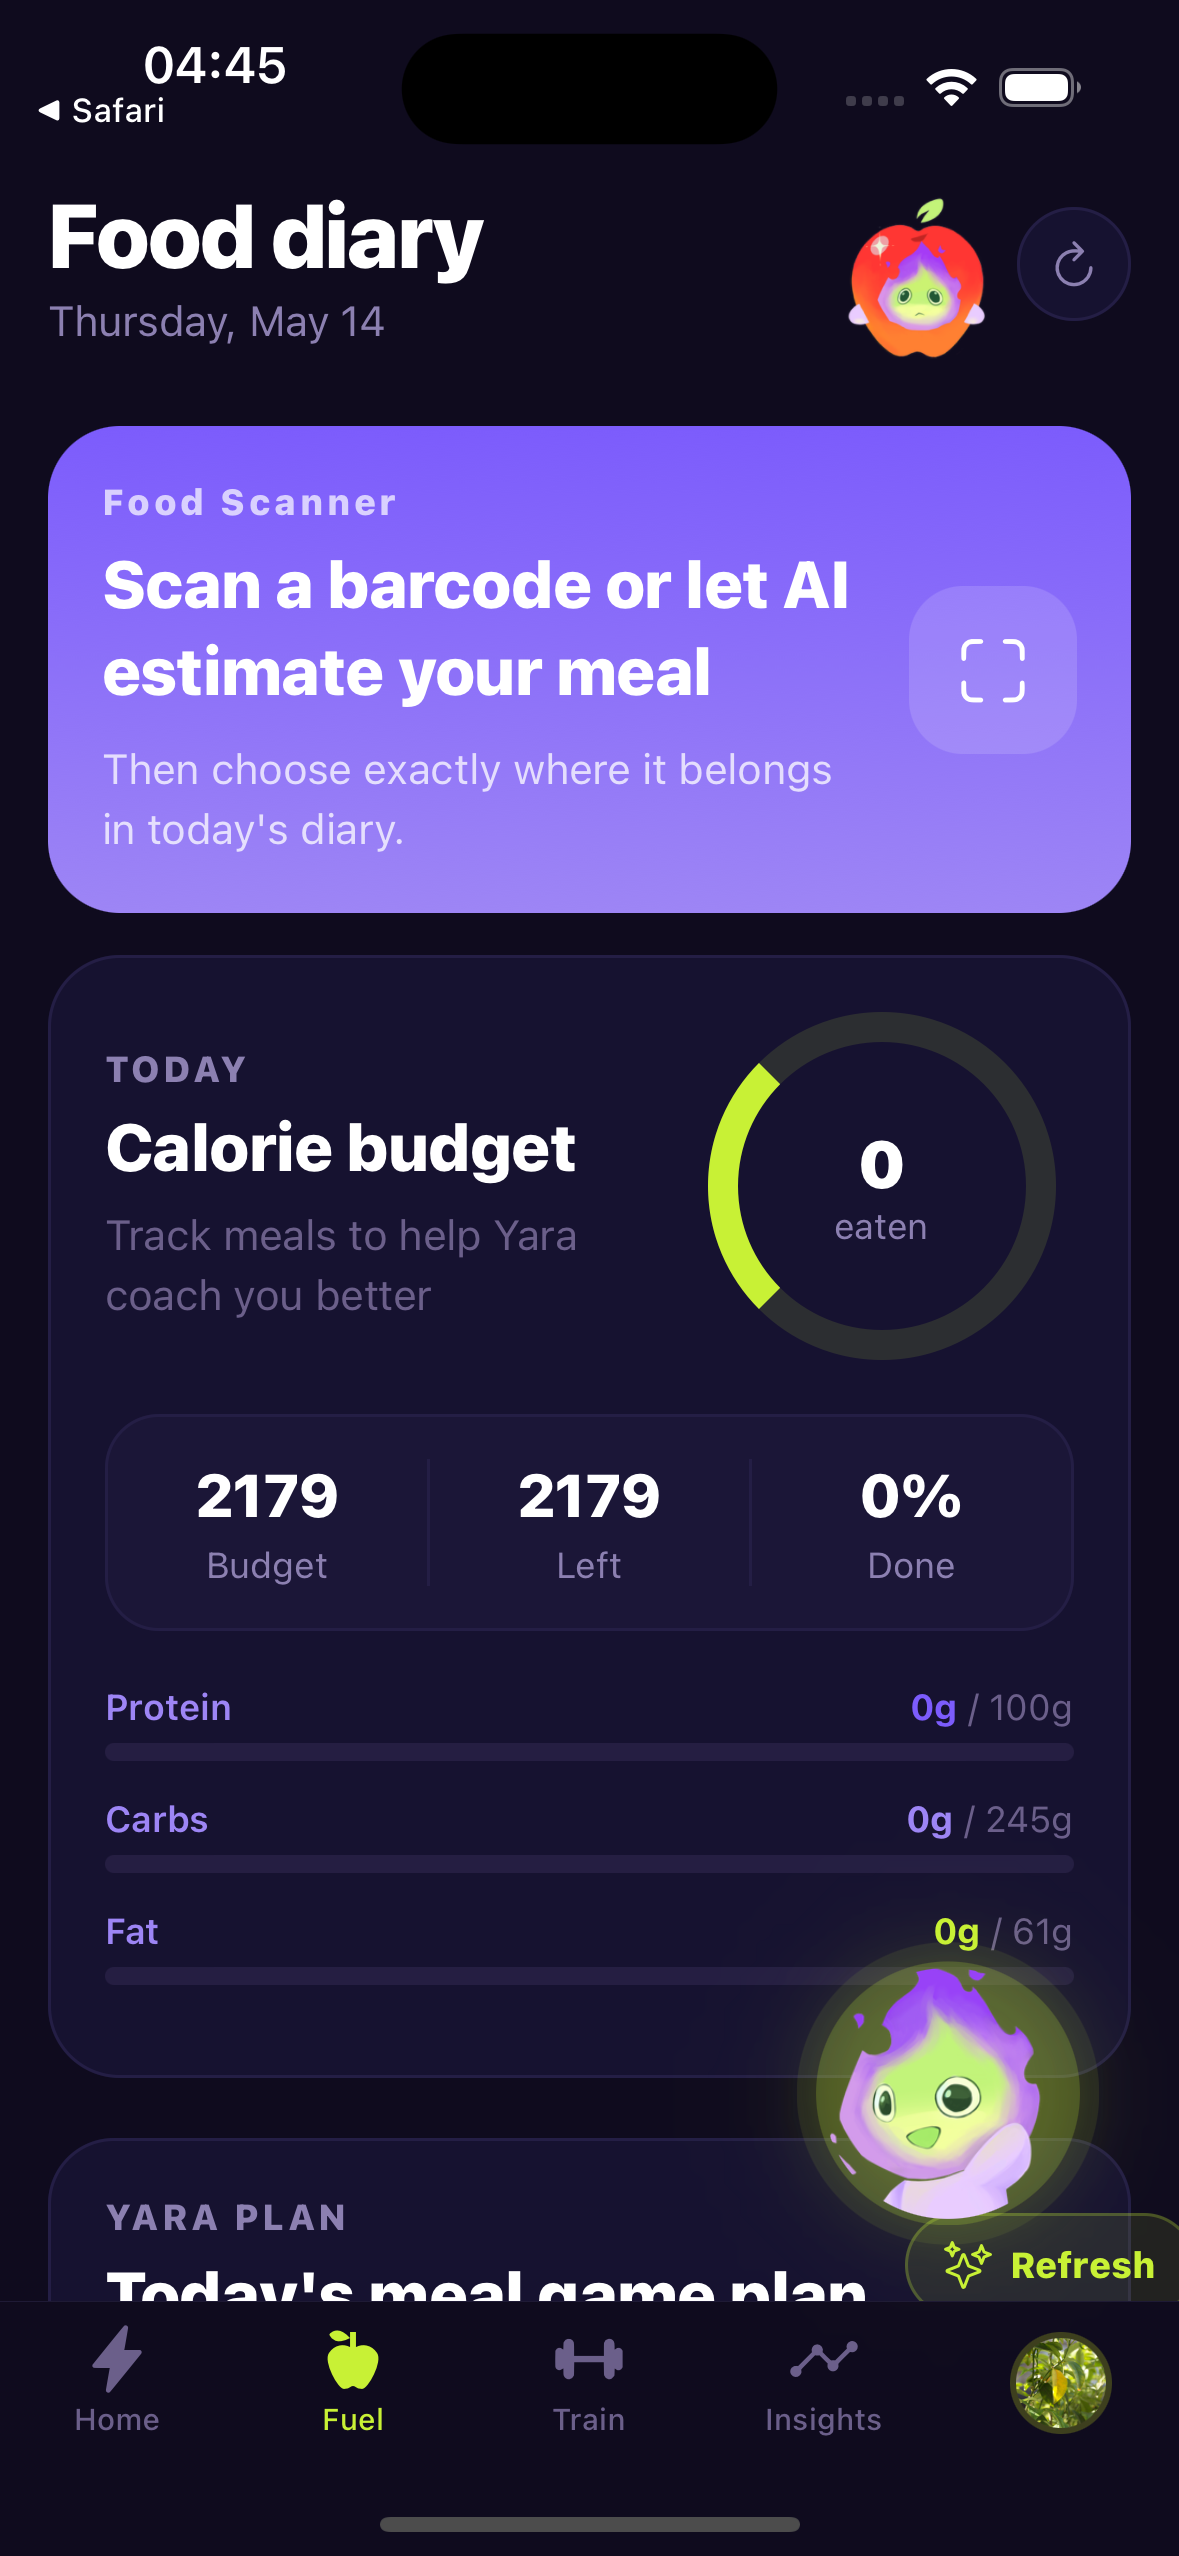
\includegraphics[width=\textwidth]{images/nutrition-screen}
		\caption{Nutrition Log}
		\label{fig:ui-fuel}
	\end{subfigure}
	
	\vspace{1.5em} % Vertical space between the two rows
	
	% --- ROW 2 ---
	\begin{subfigure}[b]{0.31\textwidth}
		\centering
		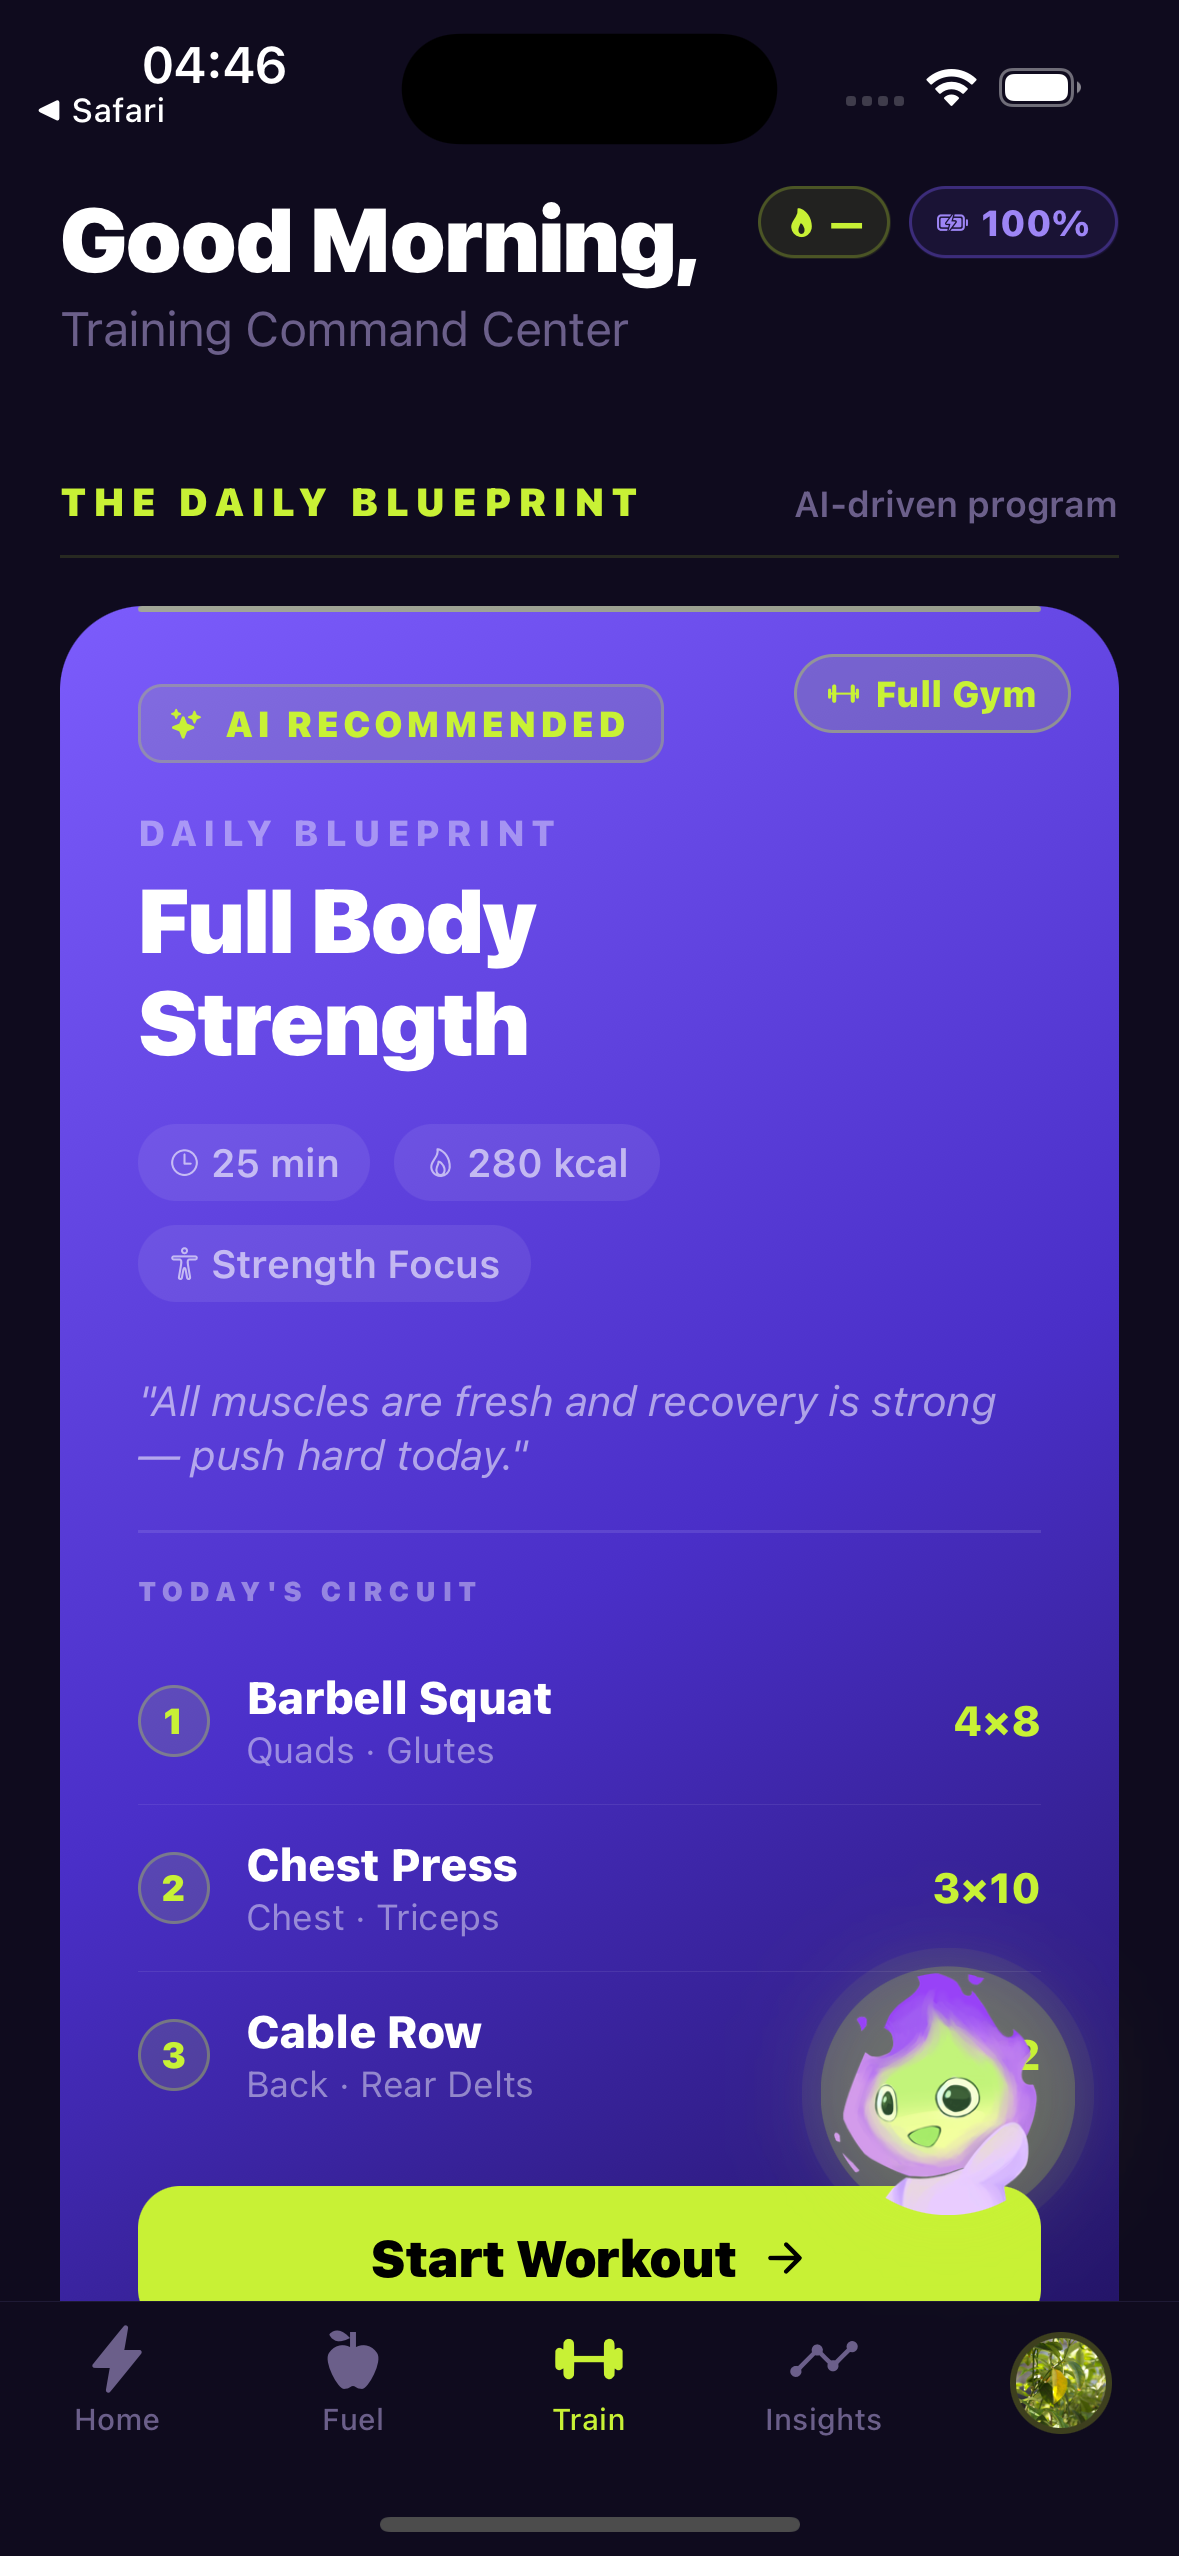
\includegraphics[width=\textwidth]{images/train-screen}
		\caption{Training}
		\label{fig:ui-train}
	\end{subfigure}
	\hfill
	\begin{subfigure}[b]{0.31\textwidth}
		\centering
		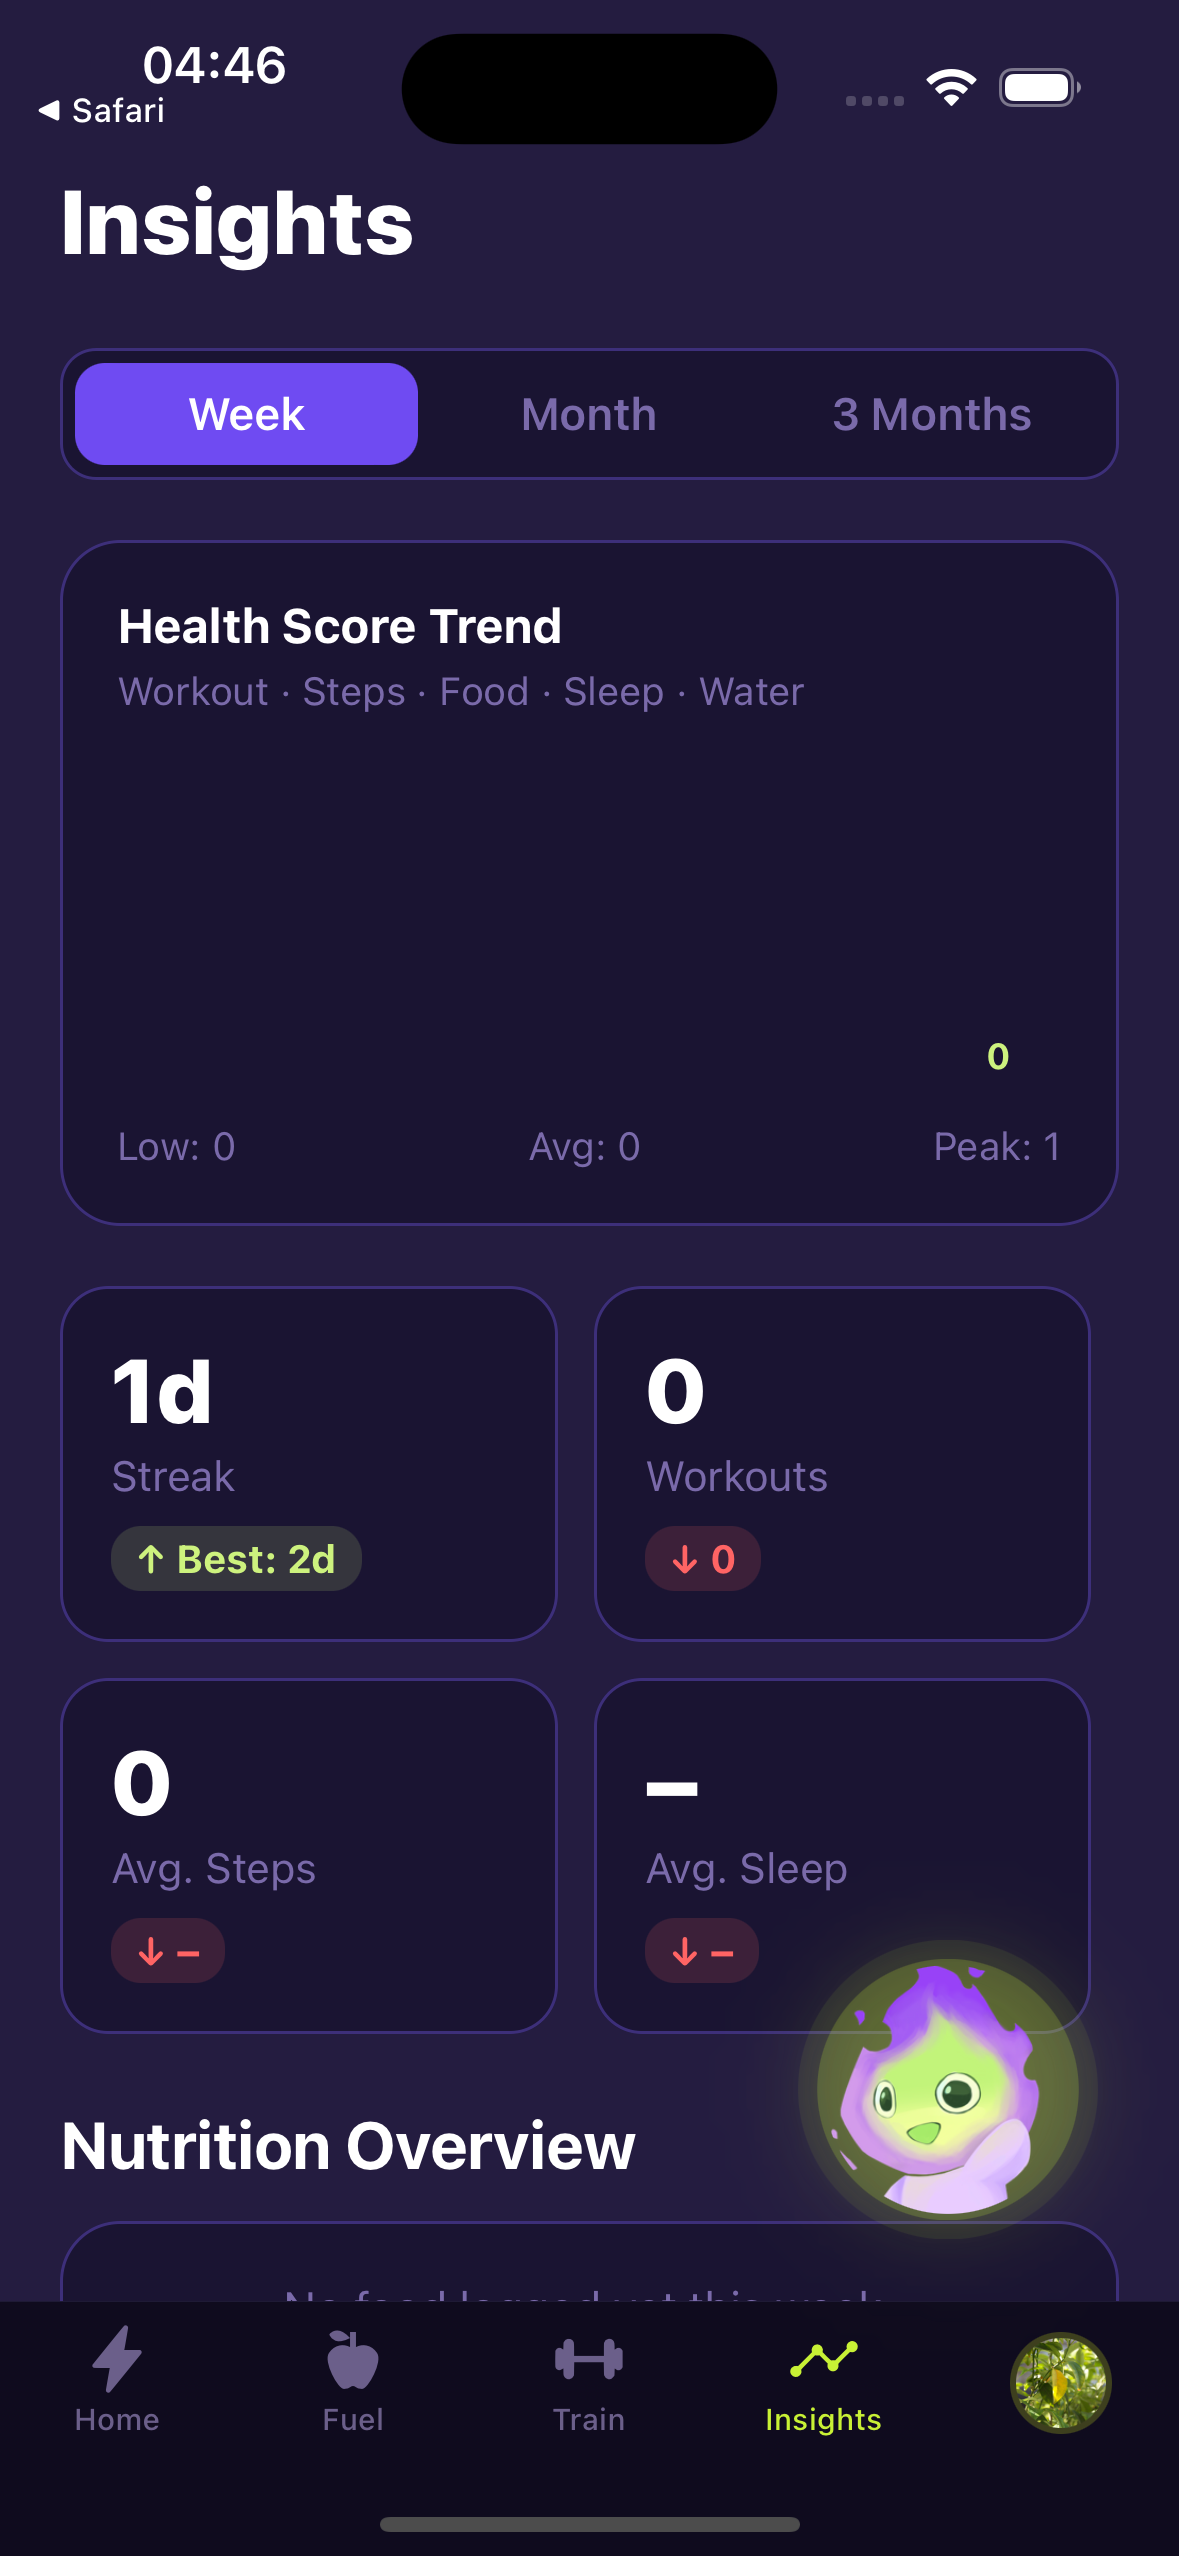
\includegraphics[width=\textwidth]{images/insights-screen}
		\caption{User Insights}
		\label{fig:ui-insight}
	\end{subfigure}
	\hfill
	\begin{subfigure}[b]{0.31\textwidth}
		\centering
		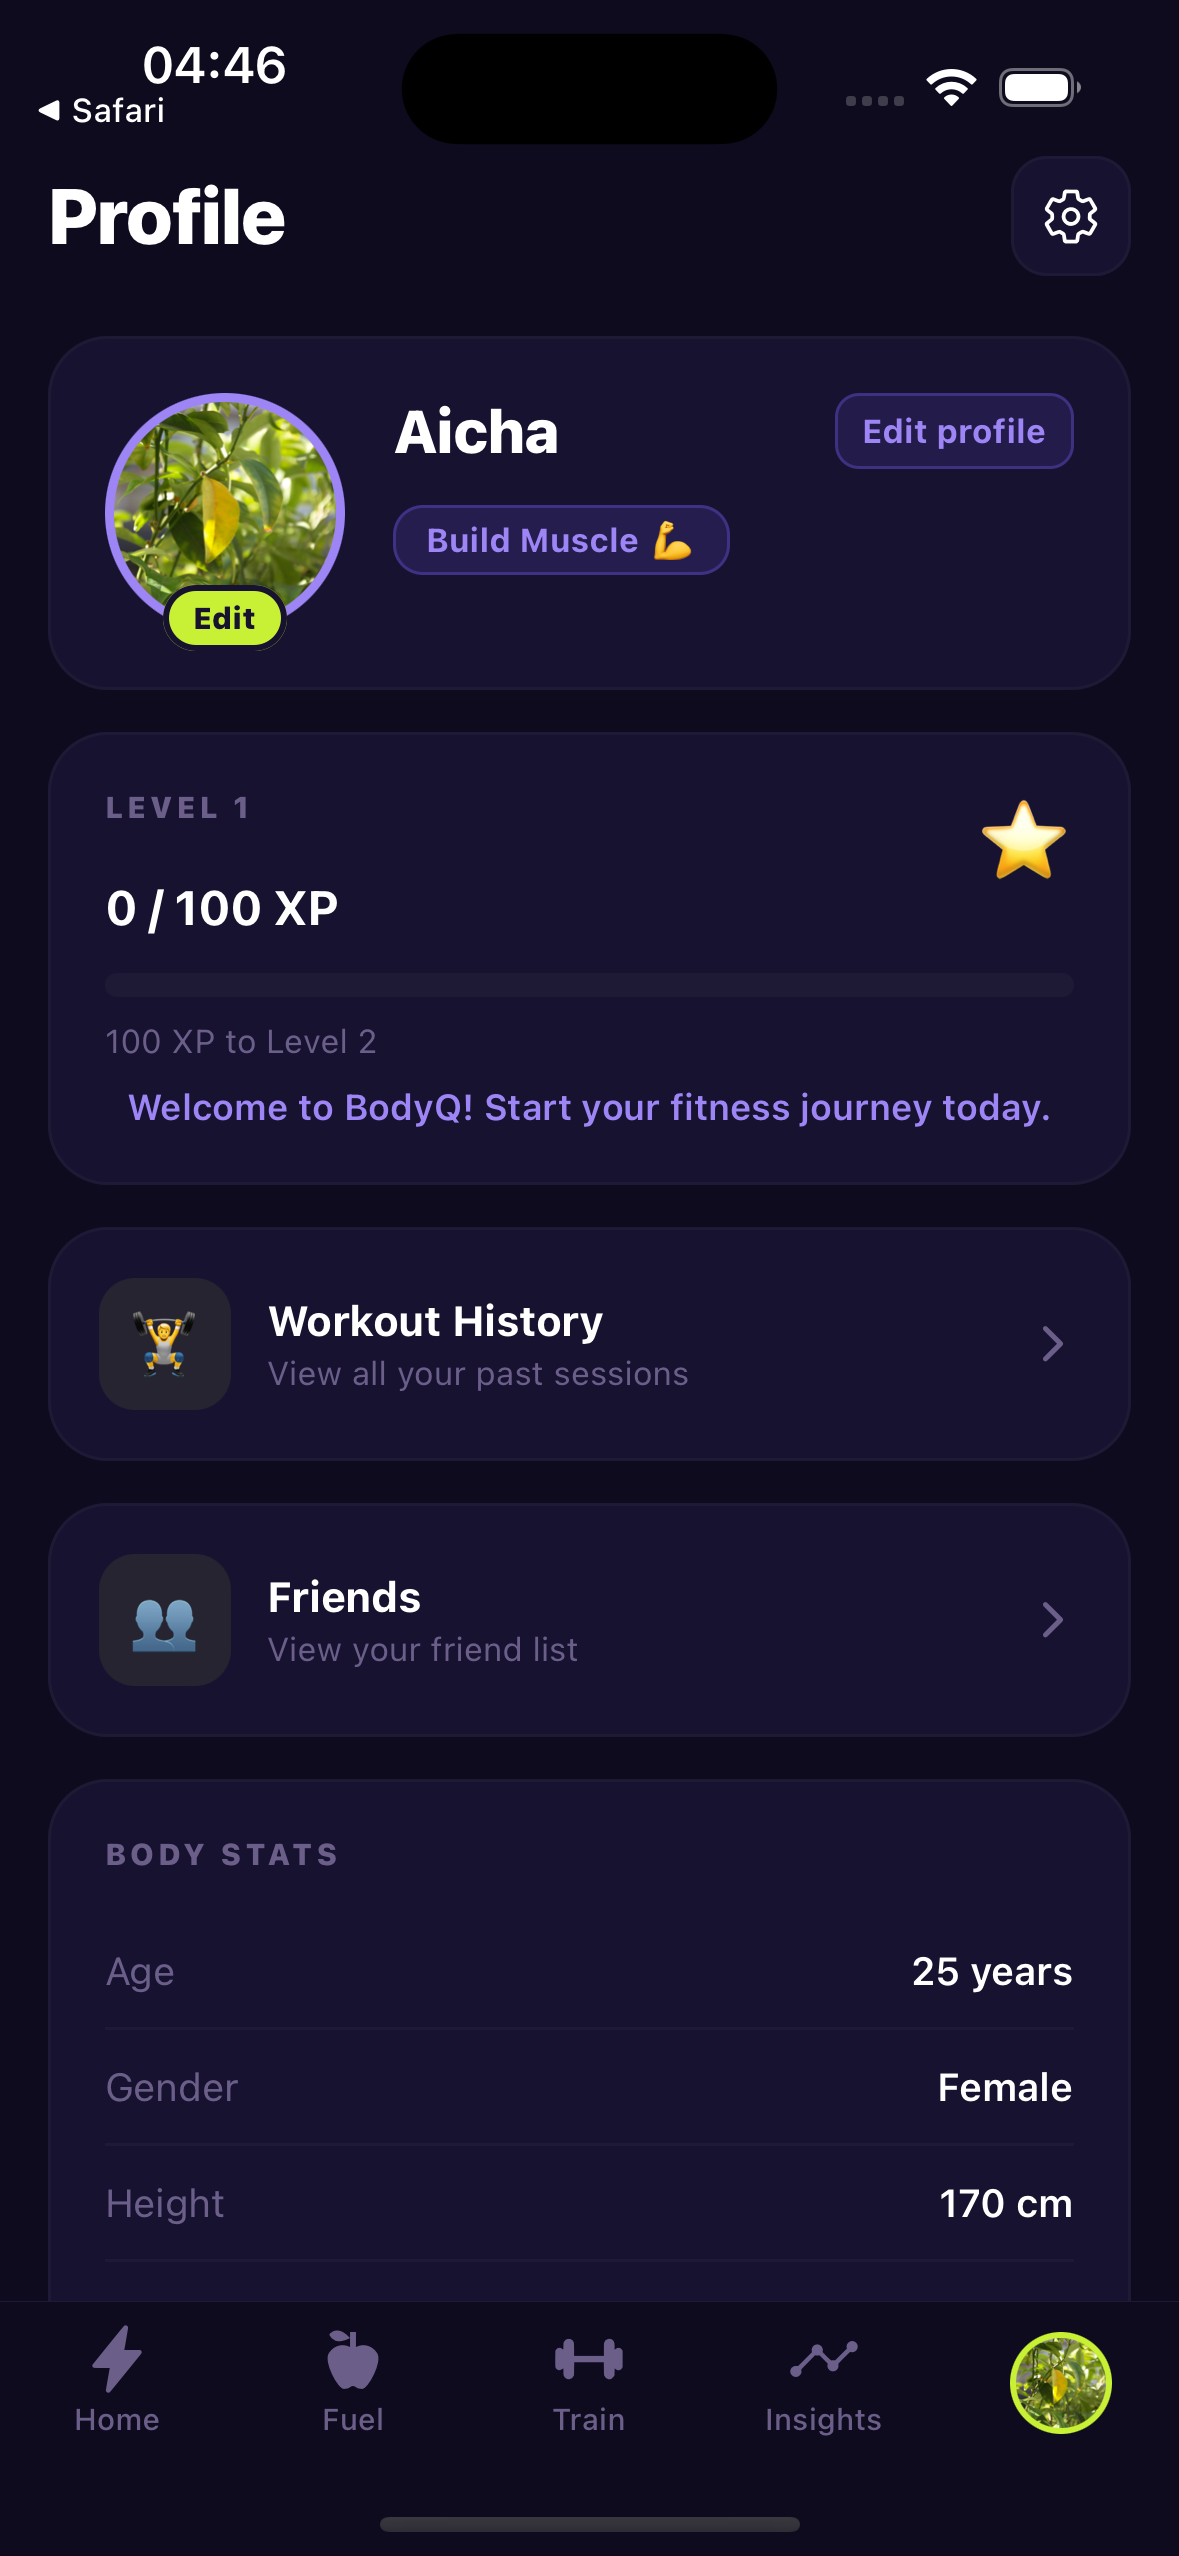
\includegraphics[width=\textwidth]{images/profile-screen}
		\caption{User Profile}
		\label{fig:ui-profile}
	\end{subfigure}
	
	\caption{Key User Interface screens of the BodyQ mobile application organized by functional area.}
	\label{fig:key-screens}
\end{figure}

\section{Conclusion}

This chapter detailed the BodyQ system design across four levels of abstraction. We established a four-tier architecture—comprising React Native, Supabase, AI Edge Functions, and a Next.js dashboard—and defined system interactions through sequence, activity, and class~ diagrams. These models captured core workflows, including onboarding, RAG-based coaching, and real-time posture detection. Finally, the UI design grounded these technical specifications in user-centric principles and key interface screens. Together, these artefacts provide the foundation for the implementation described in Chapter~4.
